\documentclass[a4paper,11pt,dvipdfmx]{jsarticle}
% 数式
\usepackage{amsmath,amsfonts,amssymb}
\usepackage{bm}
% 画像
\usepackage[dvipdfmx]{graphicx}
\usepackage[dvipdfmx]{color}
\usepackage{tabularx}
\usepackage{pifont}
\usepackage{array}
\usepackage{multicol}
\usepackage{float}
\usepackage{colortbl,array,xcolor}
\usepackage{fancybox}
\usepackage{ascmac}
\usepackage{wrapstuff}

\usepackage{geometry}
\geometry{a4paper,top=10mm,bottom=20mm,left=15mm,right=25mm}

% ハイパーリンク
\usepackage[%
dvipdfmx,% 欧文ではコメントアウトする
setpagesize=false,%
bookmarks=true,%
bookmarksdepth=tocdepth,%
bookmarksnumbered=true,%
colorlinks=false,%
pdftitle={},%
pdfsubject={},%
pdfauthor={},%
pdfkeywords={}%
]{hyperref}
\usepackage{pxjahyper}

% 2段組
\makeatletter
\def\TableCaption#1{\def\@captype{table}\caption{#1}}
\makeatother

\begin{document}
\newcolumntype{A}{>{\columncolor[gray]{0.8}}c}

\tableofcontents
\bigskip
\noindent\textbf{25年度2I前期中間過去問題集へようこそ！以下は案内です:)}
\begin{itemize}
    \item 目次の各項目をクリック又はタップすると該当の問題にジャンプします．
    \item ()内の名前は担当教師の名前であって，必ずしも問題制作者であるとは限りません．\\また，$\ast$は非常勤講師を表します．
    \item 社会2の問題用紙は回収されているため掲載していません．(一応解答だけ掲載するかも)
    \item 生物の問題用紙兼解答用紙は回収されているため掲載していません．
    \item 国語2，プログラミング1の前期中間試験は実施されていません．
    \item 解答は別冊を参照してください．
    \item 微分積分1，ベクトル・行列の問題及び解答は，別途「微積・ベクトル・行列」フォルダを参照してください．
\end{itemize}

\bigskip
\noindent\textbf{更新履歴$\circlearrowleft$} {\scriptsize(掲載完了予定：5月中旬)}
\begin{itemize}
    \item 2026/04/17 公開，マイクロコンピュータの問題を追加
    \item 2026/04/23 情報2の問題を追加
    \item 2026/04/28 英語表現2，英語3の問題を追加
\end{itemize}
\newpage

\title{}
\author{}
\date{}
\maketitle

\section{英語3(川村)}
\noindent 【1】AとBの英文について，英文の意味が通るよう，空所に入れるのに適当なものを(あ)$\sim$(く)からひとつずつ選び，記号で答えなさい．
文頭にくるものも小文字で示しています．(1点$\times$16)\\
A:\\
The news of Dr. Nakamura's death in 2019 was a great ( 1 ) to many people, both in ( 2 ) and Japan. 
However, it was ( 3 ) hard for ( 4 ) students studying in Japan, since many of them had been ( 5 ) to study in Japan by Dr. Nakamura himself. 
These students are ( 6 ) to continue Dr. Nakamura's work and to spread his way of thinking and his ( 7 ) approach to getting things done. 
They understand that planning is important, but that doing is ( 8 ) more important. 

\bigskip
  \begin{tabular}{llll}
  (あ) Afghan & (い) Afghanistan & (う) determined & (え) even\\
  (お) inspired & (か) particularly & (き) practical & (く) shock\\
  \end{tabular}
\bigskip\\
B:\\
The problem of food waste will not be ( 1 ) overnight. Laws, ( 2 ) and habits all need to change. 
( 3 ) that food waste is a big ( 4 ) to global warming is already rising, however.
The ( 5 ) of new eco-tech companies may just help to push the change a little faster by making ( 6 ) that ( 7 ) ( 8 ) food that is left over is thrown away. 

\bigskip
  \begin{tabular}{llll}
  (あ) all & (い) appearance & (う) attitudes & (え) awareness\\
  (お) contributor & (か) not & (き) solved & (く) sure\\
  \end{tabular}
\bigskip\bigskip

\noindent 【2】空所に入る語を語群から一つずつ選びなさい．文頭にくるものも小文字で示しています．(1点$\times$20)
\begin{enumerate}
  \item Sending a (\quad\quad) on the network is very easy. 
  \item The system works with only a (\quad\quad) of batteries.
  \item The goal of the race is in the (\quad\quad) of the city. 
  \item The program stopped because of an (\quad\quad).
  \item What was the (\quad\quad) number of engineers who took part in the project? 
  \item There is a red (\quad\quad) in the Japanese flag. 
  \item Put the tools in the right (\quad\quad). 
  \item The (\quad\quad) is too small to show all the information. 
  \item Put the (\quad\quad) through the tube. 
  \item Water changes into (\quad\quad) when it's heated. 
  \item You need a (\quad\quad) when you fly over the ocean. 
  \item The company's (\quad\quad) is to sell more than ten thousand cars a month. 
  \item The (\quad\quad) is driven by the motor. 
  \item If water becomes (\quad\quad), it's called ice. 
  \item Such big waves cannot be seen under (\quad\quad) conditions. 
  \item (\quad\quad) one is one less than zero. 
  \item The pictures are shown in (\quad\quad) of date. 
  \item This program controls the (\quad\quad) of the robot. 
  \item Many people think English is an (\quad\quad) language. 
  \item A hundred thousand (\quad\quad) of the book sold in a month. 
\end{enumerate}
\medskip
\begin{tabular}{|l l l l l|}
  \hline
  center&circle&compass&copies&error\\
  gas&international&message&minus&motion\\
  normal&order&pair&position&pump\\
  screen&solid&target&total&wire\\ 
  \hline
\end{tabular}
\bigskip\bigskip

\noindent 【3】次の表は英単語とその意味についてまとめたものである．(1)$\sim$(5)の空所に入る英語1語を答えなさい．
与えられているアルファベットから始める単語を答えること．(1点$\times$5)\bigskip\\
\begin{tabular}{|l|l|}
  \hline
  \multicolumn{1}{|c|}{英単語}&\multicolumn{1}{|c|}{意味} \\\hline
  consumer&a (1) (p\qquad) who buys goods or uses services \\\hline
  drought&a long period of time with no (2) (\qquad) \\\hline
  (3) (i\qquad)&a system to supply water to farms through pipes or canals \\\hline
  (4) (m\qquad)&things that are used for making something \\\hline
  well&a deep hole in the ground from which people take (5) (w\qquad) \\
  \hline
\end{tabular}
\bigskip\bigskip

\noindent 【4】日本語に合うように空所に入る英語1語をそれぞれ答えなさい．与えられているアルファベットから始まる単語を答えること．(1点$\times$10)
\begin{enumerate}
  \item 彼らはその仕事を完成させるのに1か月かかった．
  \par They took one month to (c\qquad) the work. 
  \item レストランの入口には，「上着とネクタイをお召しください」と書いてあった．
  \par By the entrance of the restaurant, it said, "A jacket and tie are (r\qquad)." 
  \item 台風だったので私たちは一日中テレビを見ながら家にいた．
  \par We stayed home, (w\qquad) TV all day because of the typhoon. 
  \item 私は彼にここに留まるように説得を試みたが，故郷に向けて出て行ってしまった．
  \par I tried to persuade him (t\qquad) stay here, but he left for his hometown. 
  \item 質問してもよろしいでしょうか．
  \par Would you mind (m\qquad) asking a question? 
  \item 私は家族にいまだに子どもだと見なされていることが嫌だ．
  \par I hate to be still (c\qquad) a child by my family.  
  \item 誰だって自分の国が戦争に巻き込まれるのを好まない．
  \par No one wants their own country to be (i\qquad) in war. 
  \item この国ではドラッグは禁止されている．
  \par Drugs are (b\qquad) in this country. 
  \item ビルが今日学校を休んだはずがない．
  \par Bill (c\qquad) have been absent from school today. 
  \item 私は日曜日いつも暇というわけではない．
  \par I am (n\qquad) always free on Sundays. 
\end{enumerate}
\bigskip\bigskip

\noindent 【5】日本語に合うよう【\quad\quad】内の語句を並び替えたとき，2番目と5番目にくるものをそれぞれ記号で答えなさい．(2点$\times$5：完答)
\begin{enumerate}
  \item その店は多くのお客で混んでいた．
  \par [ (あ) a lot\quad(い) customers\quad(う) with\quad(え) of\quad(お) crowded], the shop was doing well.
  \item 毎朝犬を散歩に連れて行くのはあなたの義務よ，ベン．
  \par Ben, [ (あ) walk\quad(い) it's\quad(う) our\quad(え) duty\quad(お) to\quad(か) your\quad(き) dog] every morning. 
  \item 彼女は夫がスポーツカーを買ってくれるのを夢見ている．
  \par She is [ (あ) a sports car\quad(い) her husband\quad(う) of\quad(え) her\quad(お) dreaming\quad(か) buying]. 
  \item この状況はあと3年は続くと見積もられている．
  \par [ (あ) last\quad(い) that\quad(う) is\quad(え) estimated\quad(お) this situation\quad(か) will\quad(き) it] another three years. 
  \item 彼女はずっと，目を閉じたままその問題について考えていた．
  \par She was thinking about the problem [ (あ) with\quad(い) for\quad(う) her\quad(え) closed\quad(お) eyes] a long time. 
\end{enumerate}
\bigskip\bigskip

\noindent 【6】各文の英文の内容が一致するよう空所に英語一語をそれぞれ入れなさい．(1点$\times$4)
\begin{enumerate}
  \item She told me to use a hairdryer to tear off the sticker. 
  \par She told me to (\qquad)(\qquad)(\qquad) a hairdryer to tear off the sticker. 
  \item We showed our thanks for her advice.
  \par We (\qquad)(\qquad)(\qquad) her advice. 
  \item These plastic bottles can be made into clothes.
  \par Clothes can (\qquad)(\qquad)(\qquad) these plastic bottles. 
  \item How can I remove this dirt?
  \par How can I (\qquad)(\qquad)(\qquad) this dirt?
\end{enumerate}
\bigskip\bigskip

\noindent 【7】会話の空所に入れるものとして最も適当なものを，(あ)$\sim$(お)から一つずつ選びそれぞれ記号で答えなさい．(1点$\times$5)\medskip\\
\begin{tabular}{l l}
  Nana:& I've never had Afghan food before.\\
  Ali:& There aren't so many Afghan restaurants in Tokyo. ( 1 ) They serve real traditional food from Afghanistan. \\
  Nana:& Living in Japan, you must miss the food.\\
  Ali:& ( 2 ) It's Palau, our national food. It's steamed rice with goat meat, nuts and fruit. \\
  Nana:& Hmm.... it looks really good.\\
  Ali:& Give it a try....\\
  Nana:& Oh, this is good.\\
  Ali:& I'm glad you like it. As you know, Afghanistan is an agricultural country. ( 3 ) \\
  Nana:& Really? ( 4 ) You need a lot of farmland and water systems for farming then? \\
  Ali:& Yes, but dry weather and floods have greatly damaged the farmlands. That's why there is not enough food,\\
  &and people are suffering from hunger. ( 5 )\\ 
  Nana:& That's terrible.\\
\end{tabular}
\bigskip\par
(あ) But this place is great.\par
(い) In fact, nearly half of Afghan children can't get enough food to eat.\par
(う) My image of Afghanistan is a war zone with dry lands.\par
(え) Oh yes, especially this first dish I ordered.\par
(お) Vegetables, rice, fruits and nuts are important products there. \\

\newpage
\noindent 【8】次の会話文を読み，問いに答えなさい．(1点$\times$5)\medskip\\
\begin{tabular}{l l}
  Hanako:& Steve, I like your T-shirt.\\
  Steve:& Thanks. Actually, I have this shirt in several colors. I have a rainbow in my closet.\\
  Hanako:& What do you mean?\\
  Steve:& I have seven different colors of T-shirts of the same design. Thanks to fast fashion shops, clothes are really\\
  &cheap. So, I can afford to buy several of them.\\
  Hanako:& But you don't need so many T-shirts, do you?\\
  Steve:& Well, I want to look fashionable.\\
  Hanako:& I'm sorry, but you're producing a lot of waste. I don't like the idea of buying so many clothes and throwing\\
  &them away too easily. It's bad for the environment.\\
  Steve:& I don't believe my T-shirts alone are doing serious damage to the earth. It's just a few shirts, you know,\\
  &for fashion.\\
  Hanako:& Come on, Steve! Being eco-friendly is much more in fashion now. Your way of thinking is not fashionable\\
  &at all! \\
\end{tabular}
\medskip\par
\begin{enumerate}
  \item What is Steve concerned about?\par
    \begin{tabular}{l l}
      (あ) Finding a rainbow.&(い) Environmental problems.\\
      (う) Being fashionable.&(え) Cleaning his room.\\
    \end{tabular}
  \bigskip
  \item What does Steve mean when he says, "I have a rainbow in my closet"?\par
    \begin{tabular}{l l}
      (あ) He has clothes with a rainbow.&(い) He has many colorful clothes.\\
      (う) He has only seven T-shirts in his closet.&(え) He likes rainbow colors.\\
    \end{tabular}
  \bigskip
  \item Why does Steve say he can afford to buy many T-shirts?\par\:
      (あ) Because his family is rich and he has a lot of money.\par\:
      (い) Because fast fashion shops sell cheap clothes.\par\:
      (う) Because he wants to wear all seven T-shirts at once.\par\:
      (え) Because he often gives his clothes to his friends.
  \bigskip
  \item What does Hanako think about Steve's habit of buying many T-shirts?\par
    \begin{tabular}{l l}
      (あ) It is a good way to look fashionable.&(い) It helps the environment.\\
      (う) It produces a lot of waste.&(え) It is very eco-friendly.\\
    \end{tabular}
  \bigskip
  \item What does Hanako say is fashionable now?\par
    \begin{tabular}{l l}
      (あ) Wearing rainbow T-shirts.&(い) Being eco-friendly.\\
      (う) Shopping at fast fashion stores.&(え) Throwing away old clothes.\\
    \end{tabular}
\end{enumerate}

\newpage
\noindent 【9】英文を読み，問いに答えなさい．(13点)\par\qquad
I was a university student when I first visited the construction site of Dr. Nakamura's canal. To dam up the river, he was using wire mesh bags filled with stones from the surrounding area instead of concrete.
When I asked him why, he explained how it is better to make use of the natural resources around us.\par\qquad
(1) \underbar{Every time I visited the construction site, what inspired me the most was Dr. Nakamura himself} \\\underbar{working as one of the workers.}
He operated the heavy machinery and carried heavy loads on his back.
He wore the same clothes as the local residents and spoke the local language fluently, so it was often difficult to find him among all the workers.
His diligence and sincerity (2)[ and / him / made / people / trust ] follow him. 
He inspired people.\par\qquad
After meeting Dr. Nakamura, I began to dream of studying in Japan, and in 2017, my dream came true.
I studied international agricultural development, (3) \underbar{mainly focusing on how to make harvested fruits or vegetables}\\\underbar{last longer}.\par\qquad
The last time I saw the doctor was in September 2018.
He encouraged me.
He said he was happy with me focusing on agricultural development.
(4) \underbar{After I completed my master's degree}, I came back to Jalalabad to teach agriculture at the university.
I want to promote Dr. Nakamura's way of thinking and help my hometown to develop.
\bigskip
\begin{enumerate}
  \item 川をせき止めるために，中村医師が使っていたものは何ですか．第1段落で述べられている情報を，過不足なく日本語でまとめなさい．(3点)\vspace{1.8cm}
  \item 下線部(1)を日本語に直しなさい．(4点)\vspace{1.8cm}
  \item (2)の[\qquad]内の語を，意味が通るよう並べ替えなさい．(2点)\vspace{1.8cm}
  \item 下線部(3)と(4)をそれぞれ次のように言い換えたとき，空所に入る語を答えなさい．(2点$\times$2：完答)
  \par (3) and mainly (\qquad)(\qquad)(\qquad) to make harvested fruits or vegetables last longer.
  \par (4) (\qquad)(\qquad)(\qquad) degree,
\end{enumerate}

\newpage
\noindent 【10】英文を読み，問いに答えなさい．(12点)\par\qquad
Reducing food waste will require a lot of effort by governments and individuals.
Less food waste is an important goal because it can lead to more efficient land use and better water resource management.
That's good for the Earth.
Also, many people on the planet do not get enough to eat.
According to the United Nations, the number is more than 820 million people.
Reducing food waste is a way to show respect for food, the farmers who produce it, the natural resources that are used to produce it, and the people who don't get enough of it.\par\qquad
Governments around the world are trying to create new laws that reduce food waste.
One of the first to do so was France.
In 2016, the French government passed a law that banned supermarkets from throwing away food.
The law required large supermarkets to work together with food rescue organizations to donate surplus food to people in need.
The government of Japan has also been considering changes to best-before date laws and laws regarding the donation of food items.
However, it's not enough to make a law.
Someone has to bring the food to the people who need or want it.\par\qquad
In recent years, new start-up companies have been trying to come up with ways to use technology to help with the problem of food waste.
In particular, they are trying to find a way to match leftover food with anyone who would like it.
One such company began operating in Denmark.
They produce an app, which is now available in many other countries, especially in Europe.
The idea is simple: it connects app users to supermarkets, restaurants, bakeries, and other stores that have unsold food.
App users get great discounts on food. The businesses get to reduce their waste, but they also get potential new customers to try their food.
Both businesses and customers contribute to a better environment.
Recently, several similar apps have appeared in Japan as well.
They make it simple for consumers in Japan to help to reduce food waste.
\bigskip
\begin{enumerate}
  \item 以下は本文中に述べられている「食品廃棄を減らす意義」について日本語でまとめたものである．それぞれの空所に入る日本語を答えなさい．(1点$\times$3)
  \par 食品廃棄を減らすことは，(\ding{172})につながる．また，食品廃棄を減らすことにより，食料，食料を生産する農家，食料を生産するために使用される天然資源，そして(\ding{173})に対して(\ding{174})．\bigskip
  \item フランスで2016年に制定された法律について，本文中に述べられている情報を，過不足なく日本語でまとめなさい．(3点)\vspace{1.8cm}
  \item デンマークで開発されたアプリについて，本文中に述べられている情報を，過不足なく日本語でまとめなさい．(6点)
\end{enumerate}
\newpage
\section{英語表現2(谷野)}
\noindent \textbf{1.  以下の英文が完成するように(\quad)内に適切な関係詞を書きなさい．}{\scriptsize(2$\times$5)}\par
(1) This is the computer (\quad\quad) Mr.Tanino uses for his research.\par\quad
  (これは谷野先生が研究に使っているパソコンです)\par
(2) You can use (\quad\quad) topic is related to Osaka or technology.\par\quad
  (大阪かテクノロジーに関連したトピックであれば，どちらでも構いません)\par
(3) You can add (\quad\quad) toppings you like to your coffee.\par\quad
  (コーヒーにはお好きなトッピングを追加できます)\par
(4) I know a shop (\quad\quad) you can eat the best ramen in Osaka.\par\quad
  (大阪で一番美味しいラーメンが食べられるお店を知っています)\par
(5) (\quad\quad) surprised me was the strong flavor of the coffee.\par\quad 
  (私を驚かせたのは，コーヒーの強い風味でした)\par
\bigskip

\noindent \textbf{2.  以下の英文が完成するように(\quad)内に適切な語句(関係詞だけとは限りません)を書きなさい．}{\scriptsize(2$\times$10)}\par
(1) I met a woman (\quad\quad) spoke French well.\par
(2) This is the book (\quad\quad) he wrote.\par
(3) This house (\quad\quad) roof is red is my uncle's.\par
(4) This is the CD (\quad\quad)(\quad\quad) I told you.\par
(5) The hotel (\quad\quad) we stayed was wonderful.\par
(6) I remember the day (\quad\quad) I first met you.\par
(7) Tell me (\quad\quad)(\quad\quad) why you were late.\par
(8) That's (\quad\quad) the accident happened.\par
(9) I don't hear (\quad\quad) she said.\par
(10) I give you (\quad\quad) you want.\par
\bigskip\bigskip

\noindent \textbf{3.  以下の(\quad)内の語を与えられた日本語を参考にして並べ替え，(\quad)内で左から\underbar{2番目と4番目}に入る語を，記}\par\textbf{号で答えなさい．文頭の文字も小文字にしています．}{\scriptsize(2$\times$5)}\par
(1) (ア. happy イ. is ウ. makes エ. Mr. Tanino オ. what) ramen.\par\quad
  谷野先生を幸せにするものはラーメンです．\par
(2) Mr. Tanino (ア. amazing イ. brews ウ. coffee エ. smells オ. which) in the morning.\par\quad
  谷野先生は朝には素晴らしい香りのコーヒーを淹れ(brew)ます．\par
(3) Mr. Tanino has (ア. a イ. for beer ウ. friend エ. inspired オ. love カ. whose) him.\par\quad
  谷野先生には，そのビール愛が彼に影響を与えた友人がいます．\par
(4) Mr. Tanino works (ア. a イ. brewer ウ. he エ. met オ. overseas カ. whom キ. with).\par\quad
  谷野先生は海外で知り合った醸造家(brewer)と働いている．\par
(5) (ア. a イ. cup ウ. is エ. offered オ. Mr. Tanino カ. visits キ. whoever) of coffee.\par\quad
  谷野先生を訪ねる人はだれでもコーヒーが提供されます．\par
\bigskip\bigskip

\noindent \textbf{4.  以下の(\quad)内の語を文法的に正しく並べ替え，(\quad)内で左から\underbar{2番目と4番目}に入る語を，記号で答えなさい．}\par\textbf{文頭の文字も小文字にしています．}{\scriptsize(2$\times$10)}\par
(1) That woman is a (ア. are イ. books ウ. selling エ. whose オ. writer) well.\par
(2) This is a (ア. built イ. house ウ. twenty years エ. was オ. which) ago.\par
(3) The (ア. are イ. dog ウ. ears エ. long オ. whose) is mine.\par
(4) This is a (ア. bought イ. by ウ. clock エ. grandfather オ. my カ. that キ. was).\par
(5) All the students (ア. are イ. English speakers ウ. from エ. good オ. graduate カ. school キ. this ク. who).\par
(6) Do you remember the year (ア. first time イ. for ウ. met エ. the オ. we カ. when)?\par
(7) They went to Canada, (ア. enjoyed イ. skiing ウ. they エ. where).\par
(8) He (ア. believe イ. say ウ. whatever エ. will オ. you).\par
(9) (ア. said イ. teacher ウ. the エ. whatever), the girl kept silent.\par
(10) My father wants to (ア. can イ. enjoy ウ. go エ. he オ. nice wine カ. wherever).\par
\bigskip\bigskip

\noindent\textbf{5.  以下の問題に答えなさい．}\par
\begin{screen}
\: Ms. Sato and her students, Leo and Mai, are discussing their upcoming school trip.\\
\begin{tabular}{l l}
  Ms. Sato&: Leo, Mai, we need to decide on an activity for our school trip. Do you have any good ideas? \\
  Leo&: Well, we could ask Mr. Yamada to give a lecture about local history. That would be \\
  &interesting.\\
  Ms. Sato&: Yes, but don't you think that it might be too much work for him? I'm not sure whether he \\
  &would have time to prepare.\\
  Mai&: How about doing something together, like a scavenger hunt, then?\\
  Ms. Sato&: That's a great idea! All of you can try finding something related to the local area, like \\
  &specific plants or landmarks.\\
  Leo&: Yes, I love scavenger hunts! Let's do that.\\
  Mai&: I agree, but we'll need to make a map in advance!\\
\end{tabular}
scavenger hunt 借り物競争
\end{screen} 
(1) What is Leo's first suggestion?\\
He suggests asking \underbar{\hspace{6cm}} .\\
(2) What does Ms. Sato think of Leo's first suggestion?\\
She thinks \underbar{\hspace{6cm}} .\\
(3) What does Mai say they'll need to do?\\
She says \underbar{\hspace{6cm}} .\\
次の問題(4)-(8)について，英文が本文の内容と合致していたらT，していなければFと答えなさい．\\
(4) Ms. Sato suggested doing a scavenger hunt for the school trip.\\
(5) Leo suggested asking Mr. Yamada to give a lecture about local history.\\
(6) Mai agreed with Leo's idea of asking Mr. Yamada to give a lecture.\\
(7) The students will need to make a map in advance for the scavenger hunt.\\
(8) Ms. Sato thought that asking Mr. Yamada to give a lecture would be too much work for him.\\

\newpage
\noindent \textbf{6.  以下の問題に答えなさい．}\par
\begin{screen}
\textbf{Review}
\begin{wrapstuff}[type = figure, width = 0.2\linewidth]
  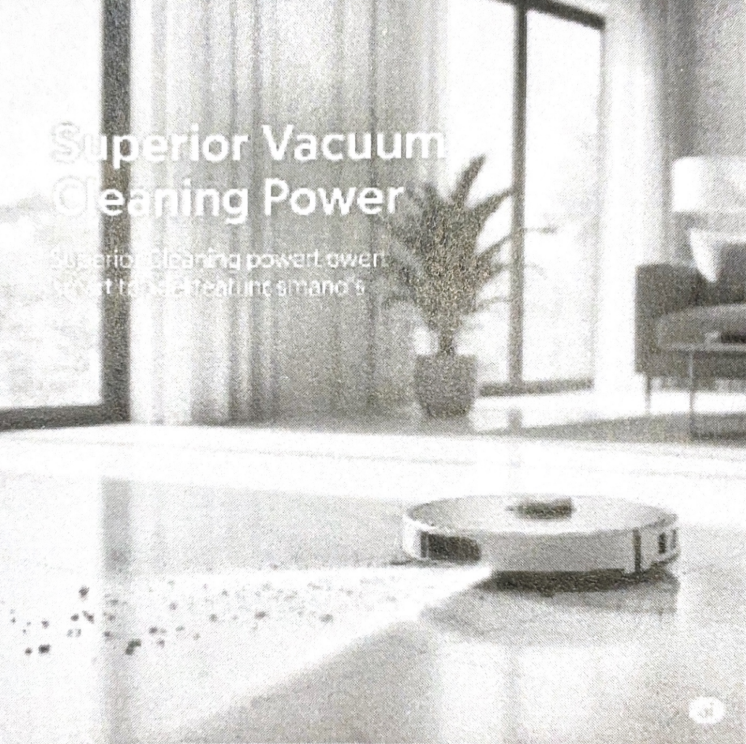
\includegraphics[width = \linewidth]{image/EngCom1.png}
\end{wrapstuff}
\colorbox{gray}{Mark ★☆☆☆☆ (terrible) Worst. Assembly. Ever.}\par
I bought this robot vacuum online, hoping to make my life easier. 
The box arrived in record time, which was a nice surprise. 
However, when I opened it, the instructions looked like they were written by a mischievous gnome who'd never seen a vacuum cleaner before! 
There were 50 tiny screws and 100 confusing diagrams. 
It said "easy assembly in 15 minutes," but after two hours, my living room looked like a robot explosion, and I was covered in sweat and tiny metal bits. 
The vacuum itself is probably great, but I'll never know because I gave up. 
I should have paid for professional assembly!
\colorbox{gray}{Sarah ★★★★☆ (good) Finally, a clean floor!}\par
I ordered this robot vacuum after seeing it advertised everywhere. 
It arrived a bit later than I expected, almost a week, but once I got it charged, it really started working its magic. 
My cat is terrified of it, which is pretty funny to watch, but my floors are spotless! 
It even goes under the sofa. 
I'm so happy I bought it, even if the delivery was a little slow.\par
\medskip
assembly (名詞) 組み立て in record time 記録的な速さで instructions (名詞) 指示，説明書\par
mischievous (形容詞) いたずらな gnome (名詞) ノーム(小人) diagrams (名詞) 図，図表\par
explosion (名詞) 爆発 terrified (形容詞) おそれた spotless (形容詞) 汚れのない，清潔な
\end{screen}
(1) What is Mark complaining about?\\
(2) What did the reviewers buy?\\
(3) What should Mark have done?\\
次の問題(4)-(8)について，英文が本文の内容と合致していたらT，していなければFと答えなさい．\\
(4) Mark was not able to assemble the robot vacuum in 15 minutes.\\
(5) Sarah received her robot vacuum in record time.\\
(6) Mark's cat was terrified of the robot vacuum. \\
(7) The robot vacuum can go under the sofa.\\
(8) Mark was satisfied with the performance of the robot vacuum.\\
\newpage
\section{化学2(吉川*)}

\newpage
\section{基礎物理2(戸塚*)}

\newpage
\section{情報2(木村)}
\noindent\begin{tabular}{|c|} % 問題1
  \hline
  問題1 \\
  \hline
\end{tabular}
次の各問いに答えよ．各2点(計64点)\\
(01) 2進数で示された「1011~0111」を10進数に変換して答えよ．\\
(02)2進数の加算「1101~0110 + 1011~1001」の計算結果を10進数に変換して答えよ．\\
(03)16進数で示された「246」を10進数に変換して答えよ．\\
(04)10進数で示した次の数値のうち「2進数による有限小数」で表現できるものをすべて答えよ．\par\quad
\ding{172}0.4\quad \ding{173}0.75\quad \ding{174}0.1\quad \ding{175}0.3125\quad \ding{176}0.5\quad \ding{177}0.25\\
(05)10進数の「-6」を2進数に変換して答えよ．なお，負数は補数表現を使ってあらわすものとして，また値を格納\par\quad するメモリは4ビットを想定すること．\\
(06)8ビットの2進数「1010~0000」の補数を答えよ．\\
(07)非負の整数値を8ビットのメモリで扱うコンピュータを考える．このコンピュータを使って10進数の計算「182\par\quad+ 74」を実行したとき，得られる結果を10進数で答えよ(オーバーフローが生じることを考慮して答えること)．\\
(08)ある実験装置の出力値を10回計測した．出力値の平均を求めたところ8.9であった．このとき，3回目に計測\par\quad された出力値10.7の「偏差」はいくらか答えよ．\\
(09)Excelにおける指数表示「3.638E + 04」を，通常の数値表示にしたときの値を答えよ．\\
(10)指定した範囲の一様乱数(整数)の生成に使われるExcel関数を答えよ．\\
(11)USBメモリは「主記憶装置」と「補助記憶装置」のどちらに分類されるか答えよ．\\
(12)相対的に製造コストが低く，大きな記憶容量を持ったRAMが求められるとき，それに適するものはSRAMと\par\quad DRAMのどちらか答えよ．\\
(13)「HDD(Hard Disk Drive)は半導体メモリである」は，適切な説明と「言える」か「言えない」か答えよ．\\
(14)コンピュータ内部において，CPUとメモリの間やCPUと入出力装置の間などで，データを受け渡す役割をす\par\quad るものを答えよ．\\
(15)次に示すRGB値のうち「黒色」を表すものはどれか答えよ．最も適切なものを記号で答えよ．\par\quad
\ding{172}(0, 255, 255)\quad \ding{173}(255, 0, 255)\quad \ding{174}(255, 255, 0)\quad \ding{175}(255, 255, 255)\quad \ding{176}(0, 0, 0)\\
(16)無圧縮形式で画素数(縦横のピクセル数)が同じ場合，フルカラー画像は，256階調グレースケール画像の約何倍\par\quad のファイルサイズになるか答えよ．\\
(17)以下の代表的な画像形式について，不可逆圧縮である画像形式をすべて答えよ．\par\quad
\ding{172}jpg(jpeg)\quad \ding{173}png\quad \ding{174}heic/heif\quad \ding{175}bmp\quad \ding{176}gif\\
(18)PhotoshopやIllustrator，Premiere Proなどのソフトウェアを開発・販売している企業は，次のうちどれか，記\par\quad 号で答えよ．\par\quad
\ding{172}Microsoft\quad \ding{173}Apple\quad \ding{174}NVIDIA\quad \ding{175}Adobe\quad \ding{176}Macromedia\quad \ding{177}Corel\\
(19)256階調のグレースケール画像において，1画素あたりの輝度を表現するために必要なデータ量は何bitか答え\par\quad よ．\\
(20)CIDR表記で「192.168.100.129/8」のとき，このサブネットマスクを10進数による表記で答えよ．\\
(21)Windowsのエクスプローラにおいて，連続しない複数のファイルを選択したい．範囲先頭のファイルをクリック\par\quad 選択した後，範囲末尾のファイルをクリック選択する際に押下すべきキーはどれか，記号で答えよ．\par\quad
\ding{172}alt\quad \ding{173}Shift\quad \ding{174}Ctrl\quad \ding{175}Tab\quad \ding{176}esc\\
(22)Windowsにおいて，IPアドレスなどのネットワーク設定の詳細情報を表示(確認)するためのコマンドを答え\par\quad よ．なお，この問題の解答では，半角スペースを\textvisiblespace の記号を使って示すこと．\\
(23)Windowsにおいて「エクスプローラ」を起動するためのショートカットキーはどれか答えよ．記号で答えよ．\par\quad
\ding{172}Win + E\quad \ding{173}Win + I\quad \ding{174}Win + W\quad \ding{175}Win + R\quad \ding{176}Win + F\\
(24)一般的な構成のノートPC(Windows 11)にUSBメモリを接続した．このUSBメモリは何ドライブとしてOS\par\quad に認識される可能性が高いか，記号で答えよ．なお，USBメモリ以外，PCにリムーバブルメディアは接続され\par\quad ていないものとする．\par\quad
\ding{172}Aドライブ\quad \ding{173}Bドライブ\quad \ding{174}Cドライブ\quad \ding{175}Dドライブ\quad \ding{176}OneDrive\\
(25)ICT分野における「LAN」とは何の頭文字をとったものか英語で答えよ．\\
(26)DNSの機能について説明しているものはどれか．最も適切なものを記号で答えよ．\par\quad
\ding{172}ネットワーク接続に際してユーザー認証をする．\par\quad
\ding{173}ネットワークに接続されたデバイスを識別する．\par\quad
\ding{174}ドメイン名とIPアドレスを対応付ける．\par\quad
\ding{175}セグメント間の通信パケットを監視・管理する．\\
(27)TCP/IP において通信相手が「同一セグメントに存在するかどうか」は，どのような情報によって判断できるか．\par\quad 最も適切なものを記号で答えよ．\par\quad
\ding{172}相手の「IPアドレス」，デフォルトゲートウェイの「IPアドレス」\par\quad
\ding{173}相手の「IPアドレス」，自分の「IPアドレス」，自分の「サブネットマスク」\par\quad
\ding{174}相手の「IPアドレス」，自分の「IPアドレス」，デフォルトゲートウェイの「IPアドレス」\par\quad
\ding{175}相手の「IPアドレス」，相手の「サブネットマスク」，自分の「IPアドレス」\\
(28)ネットワークに接続するデバイスにおいて，デフォルトゲートウェイが正しく設定されていない場合，どのような状況となるか．最も適切なものを記号で答えよ．\par\quad
\ding{172}インターネットへの接続が不可能になる．\par\quad
\ding{173}同一セグメント内のデバイスと通信ができなくなる．\par\quad
\ding{174}他セグメントにあるデバイスと通信ができなくなる．\par\quad
\ding{175}全てのデバイスと通信ができなくなる．\\
(29)インターネット全体で重複しないように一意に割り当てる必要があるのは「グローバルIPアドレス」と「プライ\par\quad ベートIPアドレス」のどちらか答えよ．\\
(30)次の運用のうち，ネットワーク経由のハッキングを受ける危険性が最も低いものはどれか．\par\quad
\ding{172}スタンドアロン\quad \ding{173}閉じた LAN に接続\quad \ding{174}インターネットに接続した LAN に接続\\
(31)Excelにおいて，範囲A1:E1の平均値を計算し，小数点第1位を切り上げた値(すなわち整数値)をセルF1に得\par\quad たい．セルF1に記述すべきExcel関数を答えよ．\\
(32)次の文章の括弧にあてはまる最も適切な言葉を漢字3文字で答えよ．「統計学では(\quad\quad\quad)から抽出した部分集\par\quad 合を標本という」\\

\noindent\begin{tabular}{|c|} % 問題2
  \hline
  問題2 \\
  \hline
\end{tabular}
次の\textbf{設定}を読み，以下の各問いに答えよ．各2点(計6点)\\
\begin{minipage}{.7\textwidth}
  \textbf{設定}\quad Windows11のPCにおいて右図のようなフォルダ構成を想定する．
  \begin{itemize}
    \item フォルダ「\textbf{1年}」の絶対パスは「\textbf{C:¥Users¥kato¥授業¥1年}」である．
    \item フォルダ「\textbf{情報2}」には，ファイル「\textbf{講義ノート01.pdf}」が存在する
    \item フォルダ「\textbf{課題}」には，ファイル「\textbf{課題\ding{172}.xlsx}」が存在する．
  \end{itemize}
(33) カレントフォルダが「\textbf{国語1}」のとき，ファイル「\textbf{課題\ding{172}.xlsx}」の絶対パス\par\qquad を答えよ．\\
(34) カレントフォルダが「\textbf{1年}」のとき，ファイル「\textbf{課題\ding{172}.xlsx}」の相対パスを\par\qquad 答えよ．なお，カレントフォルダを表す文字も省略せずに含めること．\\
\end{minipage}
\begin{minipage}{.3\textwidth}
  \hspace{0.8cm}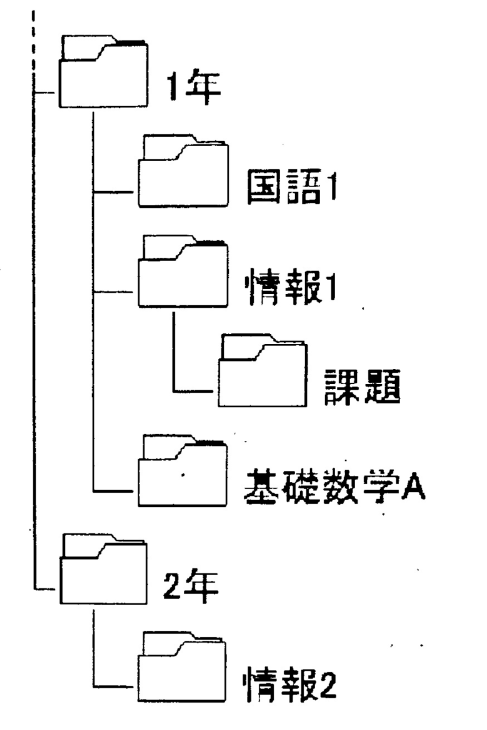
\includegraphics[width=0.7\linewidth]{image/Inf1.png}
\end{minipage}
(35) カレントフォルダが「\textbf{基礎数学A}」のとき，ファイル「\textbf{講義ノート01.pdf}」の相対パスを答えよ．なお，カレントフォルダを表す文字も省略せずに含めること．\\
\newpage

\noindent\begin{tabular}{|c|} % 問題3
  \hline
  問題3 \\
  \hline
\end{tabular}
次の各問いについて，\textbf{ア$\sim$エ}の記号で答えよ．各2点(計30点)\\
(36)文書作成ソフトや表計算ソフトなどにおいて，一連の操作手順をあらかじめ定義しておき，実行する機能はどれ\par\quad か．\par\quad
ア：オートコンプリート\quad イ：プラグアンドプレイ\quad ウ：マクロ\quad エ：ソースコード\\
(37)負の整数を「2の補数」で表現するとき，8桁の2進数で表現できる数値範囲を10進数で表したものはどれか．\par\quad
ア：-128$\sim$128\quad イ：-128$\sim$127\quad ウ：-127$\sim$128\quad エ：-127$\sim$127\\
(38)パスワードの解読方法の一つとして，全ての文字の組合せを試みる総当たり攻撃がある．"A"から"Z"の26種類\par\quad の文字を使用できるパスワードにおいて，文字数を4文字から6文字に増やすと，総当たり攻撃でパスワードを\par\quad 解読するための最大の試行回数は何倍になるか．\par\quad
ア：2\quad イ：24\quad ウ：52\quad エ：676\\
(39)Windowsにおいて，パス文字列のなかでフォルダ階層を区切るために使用する文字(記号)はどれか答えよ．\par\quad
ア：¥\quad イ：\$\quad ウ：$>$\quad エ：/\\
(40)サーバに2台のHDDを接続しているとき，HDDの故障が「どちらか片方だけ」であれば運用がつづけられる\par\quad ようにしたい．使用する構成として適切なものはどれか．\par\quad
ア：ストライピング\quad イ：ルーティング\quad ウ：テザリング\quad エ：ミラーリング\\
(41)4台のHDDを使い，障害に備えるために「1台分の容量をパリティ情報の記録に使用するRAID5」を構成する．\par\quad 1台のHDDの容量が1TBのとき，実効データ容量はおよそ何Bか．\par\quad
ア：1TB\quad イ：2TB\quad ウ：3TB\quad エ：4TB\\
(42)コンピュータハードウェアに関する文脈においてCPUとは何の略語か．次の選択肢から最も適切なものを記号\par\quad で答えよ．\par\quad
ア：Central Process Unit\par\quad
イ：Computer Processing Unit\par\quad
ウ：Central Processing Unit\par\quad
エ：Control Processing Unit\\
(43)スマートフォンなどのタッチパネルで広く採用されている方式であり，指がタッチパネルの表面に近づいたとき\par\quad に，その位置を検出する方式はどれか．\par\quad
ア：感圧式\quad イ：静電容量方式\quad ウ：電磁誘導方式\quad エ：光学式\\
(44)スキャナを使ってカラー写真のデジタル化を行う．このスキャナは解像度が300dpiで24ビットカラーの画像を\par\quad 取り込むことができる．データ圧縮を全く行わないとき，15cm$\times$10cmのカラー写真を1枚保存するためのディ\par\quad スク容量は，およそ何Mバイトか．ここでは，1(inch) = 2.5(cm)とし，1M=10の6乗とする．\par\quad 
ア：約 2MB\quad イ：約 3.5MB\quad ウ：約 5MB\quad エ：約 6.5MB\\
(45)IoTデバイスとIoTサーバで構成され，IoTデバイスが計測した外気温をIoTサーバへ送り，IoTサーバからの\par\quad 指示で窓を開閉するシステムがある．このシステムのIoTデバイスに搭載されて，窓を開閉する役割を持つもの\par\quad はどれか．\par\quad
ア：アクチュエータ\par\quad
イ：エッジコンピューティング\par\quad
ウ：キャリアアグリゲーション\par\quad
エ：センサ\\
(46)ネットワークに関する次の記述中のa$\sim$cに入れる字句の適切な組合せはどれか．\par\quad
建物内などの狭い範囲で構成されるネットワークは
\noindent\begin{tabular}{|c|}
  \hline
  a \\
  \hline
\end{tabular}
と呼ばれ，地域的に離れた地点を結ぶネットワークは\par\quad
\noindent\begin{tabular}{|c|}
  \hline
  b \\
  \hline
\end{tabular}
と呼ばれる．インターネット上で一意に割り当てられるIPアドレスは
\noindent\begin{tabular}{|c|}
  \hline
  c \\
  \hline
\end{tabular}
である．\par\quad
ア：
\noindent\begin{tabular}{|c|}
  \hline
  a \\
  \hline
\end{tabular}
LAN，
\noindent\begin{tabular}{|c|}
  \hline
  b \\
  \hline
\end{tabular}
WAN，
\noindent\begin{tabular}{|c|}
  \hline
  c \\
  \hline
\end{tabular}
グローバルIPアドレス\par\quad
イ：
\noindent\begin{tabular}{|c|}
  \hline
  a \\
  \hline
\end{tabular}
WAN，
\noindent\begin{tabular}{|c|}
  \hline
  b \\
  \hline
\end{tabular}
LAN，
\noindent\begin{tabular}{|c|}
  \hline
  c \\
  \hline
\end{tabular}
プライベートIPアドレス\par\quad
ウ：
\noindent\begin{tabular}{|c|}
  \hline
  a \\
  \hline
\end{tabular}
LAN，
\noindent\begin{tabular}{|c|}
  \hline
  b \\
  \hline
\end{tabular}
WAN，
\noindent\begin{tabular}{|c|}
  \hline
  c \\
  \hline
\end{tabular}
プライベートIPアドレス\par\quad
エ：
\noindent\begin{tabular}{|c|}
  \hline
  a \\
  \hline
\end{tabular}
WAN，
\noindent\begin{tabular}{|c|}
  \hline
  b \\
  \hline
\end{tabular}
LAN，
\noindent\begin{tabular}{|c|}
  \hline
  c \\
  \hline
\end{tabular}
グローバルIPアドレス\\\newpage
(47)サブネットマスクの役割として，適切なものはどれか．\par\quad
ア：IPアドレスからEthernet上のMACアドレスを割り出す．\par\quad
イ：通信相手先の「ドメイン名」と「IPアドレス」を対応付ける．\par\quad
ウ：インターネットと内部ネットワークを中継するときの「グローバルIPアドレス」と「プライベートIPアド\par\quad\quad\quad レス」を対応付ける．\par\quad
エ：IPアドレスに含まれる「ネットワークアドレス」と，そのネットワークに属する個々のコンピュータの「ホ\par\quad\quad\quad ストアドレス」を区分する．\\
(48)表計算ソフトを用いて2つの科目XとYの点数を評価して合否判定をする．それぞれの点数はワークシートの\par\quad セルA2とB2に入力する．合格判定条件\ding{172}または\ding{173}に該当するときはセルC2に「合格」，それ以外のときは\par\quad「不合格」を表示したい．セルC2に入力すべき式はどれか．\par\:
〔合格判定条件〕\par\quad\:
\ding{172} 科目Xと科目Yの合計が150点以上である．\par\quad\:
\ding{173} 科目Xと科目Yがともに70点以上である．\vspace{0.2cm}\\\hspace{0.8cm}
  \renewcommand{\arraystretch}{0.8}
  \noindent\begin{tabular}{|A|
    >{\centering\arraybackslash}m{0.09\linewidth}|
    *{3}{>{\centering\arraybackslash}m{0.09\linewidth}|}
  }
  \rowcolor[gray]{0.8}
    \hline
    & A & B & C \\ \hline
    1 & 科目X & 科目Y & 合否 \\ \hline
    2 & 50 & 80 &  \\ \hline
  \end{tabular}
\vspace{0.2cm}
\par\:
ア：IF(論理和((A2+B2)≧150, 最大(A2, B2)≧70), '合格', '不合格')\par\:
イ：IF(論理和((A2+B2)≧150, 最小(A2, B2)≧70), '合格', '不合格')\par\:
ウ：IF(論理積((A2+B2)≧150, 最大(A2, B2)≧70), '合格', '不合格')\par\:
エ：IF(論理積((A2+B2)≧150, 最小(A2, B2)≧70), '合格', '不合格')\\
(49)表計算ソフトを用いてワークシートに示す各商品の月別売上額データを用いた計算を行う．セルE2に式「条件付個数(\$B\$2:\$D\$2,>10000)」を入力した後，セルE3とE4に複写したとき，セルE4に表示される値はどれか．
\vspace{0.2cm}\\\hspace{2.5cm}
    \renewcommand{\arraystretch}{0.8}
    \noindent\begin{tabular}{|A|
      >{\centering\arraybackslash}m{0.09\linewidth}|
      *{5}{>{\centering\arraybackslash}m{0.12\linewidth}|}
    }
    \rowcolor[gray]{0.8}
      \hline
      & A & B & C & D & E \\ \hline
      1 & 商品名 & 1月売上額 & 2月売上額 & 3月売上額 & 条件付個数 \\ \hline
      2 & 商品A & 30,000 & 15,000 & 20,000 & \\ \hline
      3 & 商品B & 5,000 & 10,000 & 5,000 & \\ \hline
      4 & 商品C & 10,000 & 20,000 & 10,000 & \\ \hline
    \end{tabular}
  \vspace{0.2cm}
\par\:
ア：0\quad イ：1\quad ウ：2\quad エ：3\\
(50)水田の水位を計算することによって，水田の水門を自動的に開閉するIoTシステムがある．図中の
\noindent\begin{tabular}{|c|}
  \hline
  a \\
  \hline
\end{tabular}
，
\noindent\begin{tabular}{|c|}
  \hline
  b \\
  \hline
\end{tabular}
に入れる字句の適切な組合せはどれか．\\
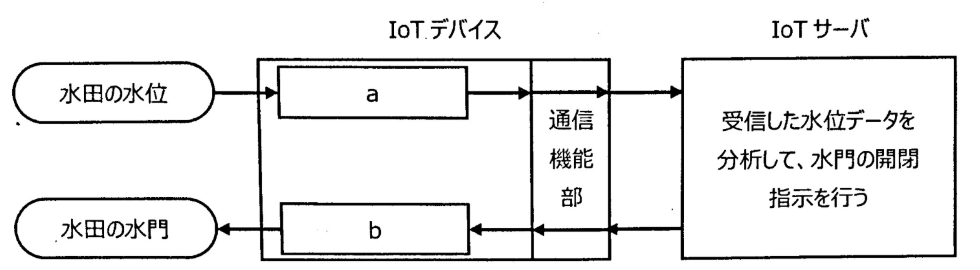
\includegraphics[width=\linewidth]{image/Inf2.png}

\par\quad ア：
\noindent\begin{tabular}{|c|}
  \hline
  a \\
  \hline
\end{tabular}
アクチュエータ
\noindent\begin{tabular}{|c|}
  \hline
  b \\
  \hline
\end{tabular}
IoTゲートウェイ\par\quad
イ：
\noindent\begin{tabular}{|c|}
  \hline
  a \\
  \hline
\end{tabular}
アクチュエータ
\noindent\begin{tabular}{|c|}
  \hline
  b \\
  \hline
\end{tabular}
センサ\par\quad
ウ：
\noindent\begin{tabular}{|c|}
  \hline
  a \\
  \hline
\end{tabular}
センサ
\noindent\begin{tabular}{|c|}
  \hline
  b \\
  \hline
\end{tabular}
IoT ゲートウェイ\par\quad
エ：
\noindent\begin{tabular}{|c|}
  \hline
  a \\
  \hline
\end{tabular}
センサ
\noindent\begin{tabular}{|c|}
  \hline
  b \\
  \hline
\end{tabular}
アクチュエータ\\



\noindent\renewcommand{\arraystretch}{1.8}
  \begin{tabular}{|m{0.33\linewidth}|m{0.33\linewidth}|m{0.33\linewidth}|}
      \hline
      \quad\quad(01)&\:\:\:(02)&\:\:\:(03) \\ \hline
      \quad\quad(04)&\:\:\:(05)&\:\:\:(06) \\ \hline
      \quad\quad(07)&\:\:\:(08)&\:\:\:(09) \\ \hline
      \quad\quad(10)&\:\:\:(11)&\:\:\:(12) \\ \hline
      \quad\quad(13)&\:\:\:(14)&\:\:\:(15) \\ \hline
      \quad\quad(16)&\:\:\:(17)&\:\:\:(18) \\ \hline
      \quad\quad(19)&\:\:\:(20)&\:\:\:(21) \\ \hline
      \quad\quad(22)&\:\:\:(23)&\:\:\:(24) \\ \hline
      \quad\quad(25)&\:\:\:(26)&\:\:\:(27) \\ \hline
      \quad\quad(28)&\:\:\:(29)&\:\:\:(30) \\ \hline
      \quad\quad(31)&\:\:\:(32)& \\ \hline
      \multicolumn{3}{|m{\linewidth}|}{(33)} \\ \hline
      \multicolumn{3}{|m{\linewidth}|}{(34)} \\ \hline
      \multicolumn{3}{|m{\linewidth}|}{(35)} \\ \hline
      \quad\quad(36)&\:\:\:(37)&\:\:\:(38) \\ \hline
      \quad\quad(39)&\:\:\:(40)&\:\:\:(41) \\ \hline
      \quad\quad(42)&\:\:\:(43)&\:\:\:(44) \\ \hline
      \quad\quad(45)&\:\:\:(46)&\:\:\:(47) \\ \hline
      \quad\quad(48)&\:\:\:(49)&\:\:\:(50) \\ \hline
    \end{tabular}
\newpage
\section{マイクロコンピュータ(青木)}
\noindent\large{\textbf{問1}}\quad 
  i=3,j=3,k=7の場合，次の式の結果を真(true)，偽(false)で答えなさい．\medskip\\
    \begin{tabular}{|
      >{\centering\arraybackslash}m{0.15\linewidth}|
      *{4}{>{\centering\arraybackslash}m{0.20\linewidth}|}
  }
      \hline
      \rule{0pt}{12pt} 式 & $i=j$ & $j!=k$ & $i<=j$ & $j>k$ \\ \hline
      \rule{0pt}{24pt} 式の結果 &  &  &  &  \\ \hline
    \end{tabular}
  \bigskip

\noindent\large{\textbf{問2}}\quad 
  x=5, y=10の場合，次の式の結果，xに代入される値を答えなさい．\medskip\\
    \begin{tabular}{|
        >{\centering\arraybackslash}m{0.15\linewidth}|
        *{3}{>{\centering\arraybackslash}m{0.20\linewidth}|}
    }
        \hline
        \rule{0pt}{12pt} 式 & $x=y++;$ & $x=y--;$ & $x+=10;$ \\ \hline
        \rule{0pt}{24pt} 式の結果 &  &  &  \\ \hline
    \end{tabular}
  \bigskip

\noindent\large{\textbf{問3}}\quad 
  次の文章の【】の中に適する言葉や関数を入れ，文章を完成させなさい．\\
  (a)【\ding{172}】制御は，LEDが点灯する明るさを変化させたい場合などに用いられ，\par
  ArduinoのD5ポートに接続したLEDをデューティ比80\%で【\ding{172}】制御により\par 
  点灯させるための関数は，【\ding{173}】となる．\\
  (b)1$\sim$1000の範囲の変数xに対し，Serial.println(100/1024*x)を実行するとxの\par
  値に関わらずシリアルモニタに表示されるのは0となる．0以外の計算結果を\par 
  表示するには，関数を【\ding{174}】に変更する．\medskip\\
  \renewcommand{\arraystretch}{1.5}
    \begin{tabular}{|m{0.33\linewidth}|m{0.66\linewidth}|}
    \hline
    \:\:\:\ding{172}&\:\:\:\ding{173} \\ \hline
    \multicolumn{2}{|m{\linewidth}|}{\ding{174}} \\ \hline
    \end{tabular}
  \bigskip

\noindent\large{\textbf{問4}}\quad 
  図(a)，(b)に示すマイコンの入力ピンに接続されたスイッチ入力回路に\par\quad ついて次の問いに答えなさい．\\
  (1)スイッチ(SW)のON，OFFに対して入力ピンに入力される電圧を答えな\par さい．
  \begin{figure}[H]
  \begin{minipage}{.4\textwidth}
    % \resizebox{0.45\linewidth}{!}{%
    \begin{tabular}{|
      >{\centering\arraybackslash}m{0.2\linewidth}|
      >{\centering\arraybackslash}m{0.38\linewidth}|
      >{\centering\arraybackslash}m{0.38\linewidth}|
    }
    \hline
    SW & 図(a)の入力電圧 & 図(b)の入力電圧 \\ \hline
    ON & & \\ \hline
    OFF & & \\ \hline
    \end{tabular}
    % }
  \end{minipage}
  \hfill
  \begin{minipage}{.4\textwidth}
    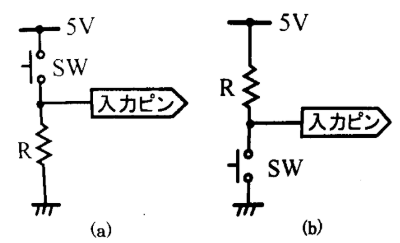
\includegraphics[width=\linewidth]{image/MicroCon1.png}
  \end{minipage}
  \end{figure}
  \medskip

  \noindent(2)プルアップと呼ばれる回路は(a)と(b)のどちらか答えなさい．
  \hfill
    \begin{tabular}{|c|}
    \hline
    答~~~~~~~~~~ \\
    \hline
    \end{tabular}
  \bigskip

  \begin{figure}[H]
  \begin{minipage}{.7\textwidth}
  \noindent\large{\textbf{問5}}\quad
  右図に示す5[V]の電源に接続されたLEDがある．\par\quad\quad
  点灯時のLEDの電圧降下(順方向電圧)が2.1[V]で，\par\quad\quad
  LEDに流す電流(順方向電流)が10[mA]とした場合\par\quad\quad
  の電流制限抵抗Rの値を求めなさい．\\
  \newline
  \hfill
    \begin{tabular}{|c|}
    \hline
    答~~~~~~~~~~~~~~~~~~~~ \\
    \hline
    \end{tabular}
  \end{minipage}
  \hfill
  \begin{minipage}{.2\textwidth}
    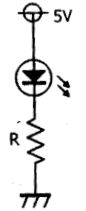
\includegraphics[width=0.55\linewidth]{image/MicroCon2.png}
  \end{minipage}
  \end{figure}
  \bigskip

\begin{figure}[H]
\begin{minipage}{.6\textwidth}
  \noindent\large{\textbf{問6}}\quad
  図1のようにArduinoのD8$\sim$D11ピンに\par\quad\quad
  LEDを接続した場合に，表1に示すように点\par\quad\quad
  灯した2個のLEDが1秒ごとに移動する\par\quad\quad
  プログラムを□を埋めて完成させなさい．\medskip\\
  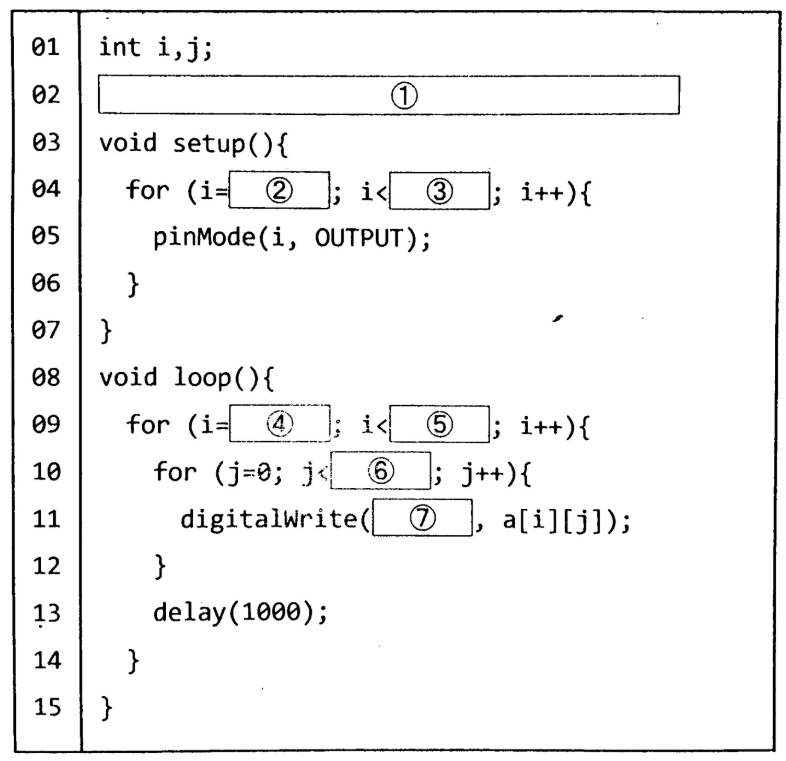
\includegraphics[width=0.95\linewidth]{image/MicroCon3.png}
\end{minipage}
\hfill
\begin{minipage}{.5\textwidth}
  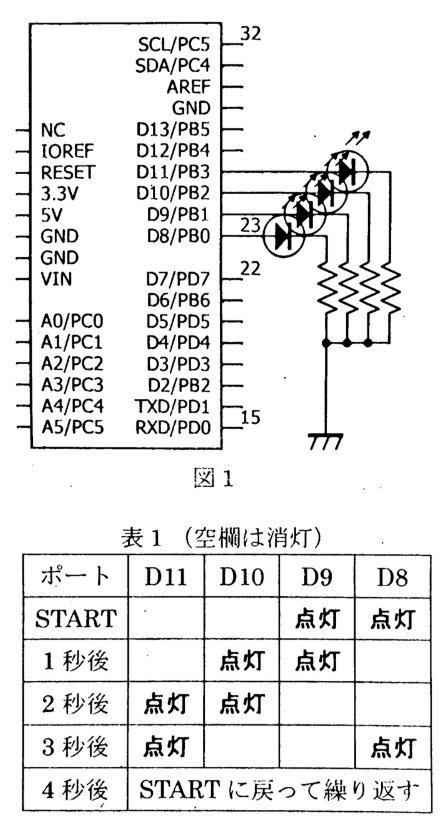
\includegraphics[width=0.85\linewidth]{image/MicroCon4.png}
\end{minipage}
\end{figure}

  \renewcommand{\arraystretch}{1.5}
    \begin{tabular}{|m{0.33\linewidth}|m{0.33\linewidth}|m{0.33\linewidth}|}
    \hline
    \multicolumn{3}{|m{\linewidth}|}{\ding{172}} \\ \hline
    \quad\:\:\:\ding{173}&\:\:\:\ding{174}&\:\:\:\ding{175} \\ \hline
    \quad\:\:\:\ding{176}&\:\:\:\ding{177}&\:\:\:\ding{178} \\ \hline
    \end{tabular}
  \bigskip

  \begin{figure}[H]
  \begin{minipage}{.7\textwidth}
  \noindent\large{\textbf{問7}}\quad
  右図のようにArduinoのD3ピンに接続された\par\quad\quad
  スイッチとD13ピンに接続されているオンボード\par\quad\quad
  LEDに対して，スイッチがOFFのときLEDが\par\quad\quad
  0.5秒周期で点滅(0.25秒間点灯，0.25秒間消灯)し，\par\quad\quad
  スイッチがONのときLEDが点灯するプログラム\par\quad\quad
  を作成しなさい．\\
  \end{minipage}
  \hfill
  \begin{minipage}{.2\textwidth}
    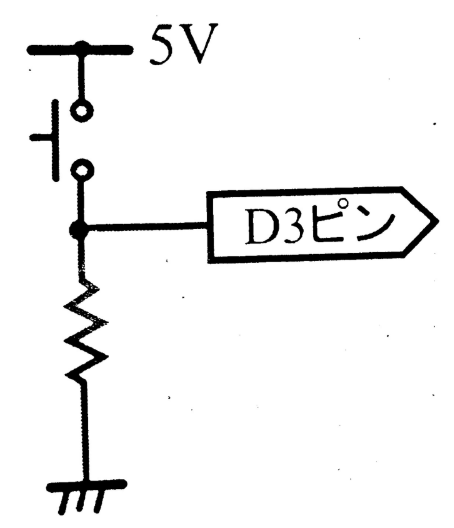
\includegraphics[width=1.4\linewidth]{image/MicroCon5.png}
  \end{minipage}
  \end{figure}
  \bigskip\bigskip\bigskip\bigskip\bigskip\bigskip
  \bigskip\bigskip\bigskip\bigskip\bigskip\bigskip
  \bigskip\bigskip\bigskip

\noindent\large{\textbf{問8}}\quad 
  図2のようにArduinoのD10ピンにLEDを接続し，D2$\sim$D3ピンにスイッ\par\quad チを接続した回路がある．
  □を埋めて以下の条件を満たすプログラムを完成\par\quad させなさい．
  なお，スイッチに抵抗が接続されていないことを考慮して，スイ\par\quad ッチの入力に対してプルアップ設定をしたプログラムを作成すること．\\
  【条件】
  \begin{itemize}
    \item 電源投入時，LEDは2秒周期で点滅する
    \item SW0が，ONのときLEDの点滅周期が100msずつ短くなり，OFFのとき点滅周期に変化はない
    \item SW1が，ONのときLEDの点滅周期が100msずつ長くなり，OFFのとき点滅周期に変化はない
    \item SW0とSW1が同時にONになることはない
    \item 点滅周期の最大値は10秒，最小値は100msとする
    \item 点滅周期は，1回の点灯時間と消灯時間をあわせた時間とする
  \end{itemize}

  \begin{figure}[H]
  \begin{minipage}{.6\textwidth}
    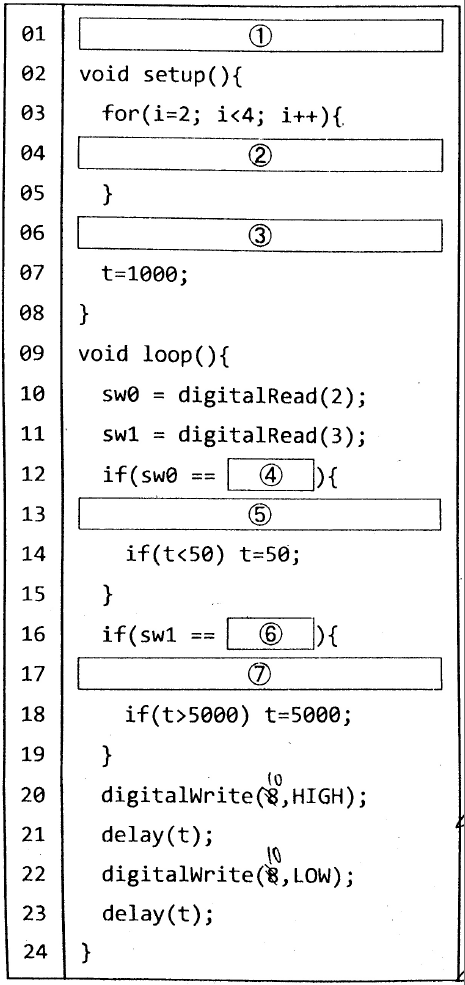
\includegraphics[width=0.8\linewidth]{image/MicroCon6.png}
  \end{minipage}
  \hfill
  \begin{minipage}{.4\textwidth}
    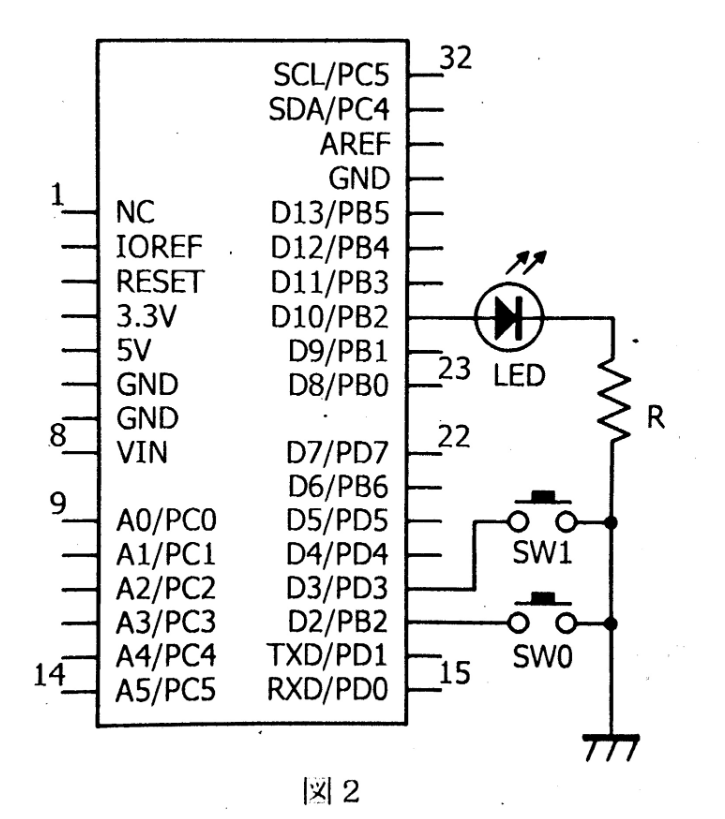
\includegraphics[width=1.1\linewidth]{image/MicroCon7.png}
    \medskip
    \renewcommand{\arraystretch}{2}
      \begin{tabular}{|m{0.33\linewidth}|m{0.33\linewidth}|m{0.33\linewidth}|}
      \hline
      \multicolumn{3}{|m{\linewidth}|}{\ding{172}} \\ \hline
      \multicolumn{3}{|m{\linewidth}|}{\ding{173}} \\ \hline
      \multicolumn{3}{|m{\linewidth}|}{\ding{174}} \\ \hline
      \multicolumn{3}{|m{\linewidth}|}{\ding{175}} \\ \hline
      \multicolumn{3}{|m{\linewidth}|}{\ding{176}} \\ \hline
      \multicolumn{3}{|m{\linewidth}|}{\ding{177}} \\ \hline
      \end{tabular}
  \end{minipage}
  \end{figure}
  \bigskip
  \newpage

\noindent\large{\textbf{問9}}\quad 
以下に示すプログラムがそれぞれ実行された場合，シリアルモニタに表示\par\quad される文字列を答えなさい．
\begin{center}  
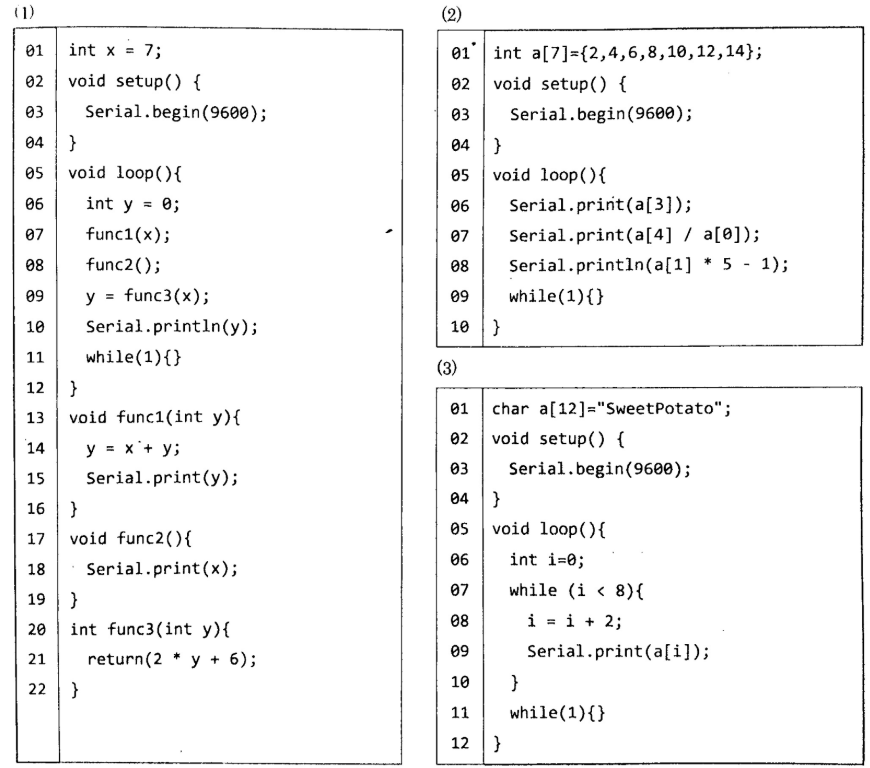
\includegraphics[width=0.9\linewidth]{image/MicroCon8.png}
\end{center}
  \begin{tabular}{|m{0.5\linewidth}|m{0.5\linewidth}|}
    \hline
    \:\:\:(1)&\:\:\:(2) \\ \hline
    \:\:\:(3)&\\ \hline
  \end{tabular}
  \bigskip

\begin{center}
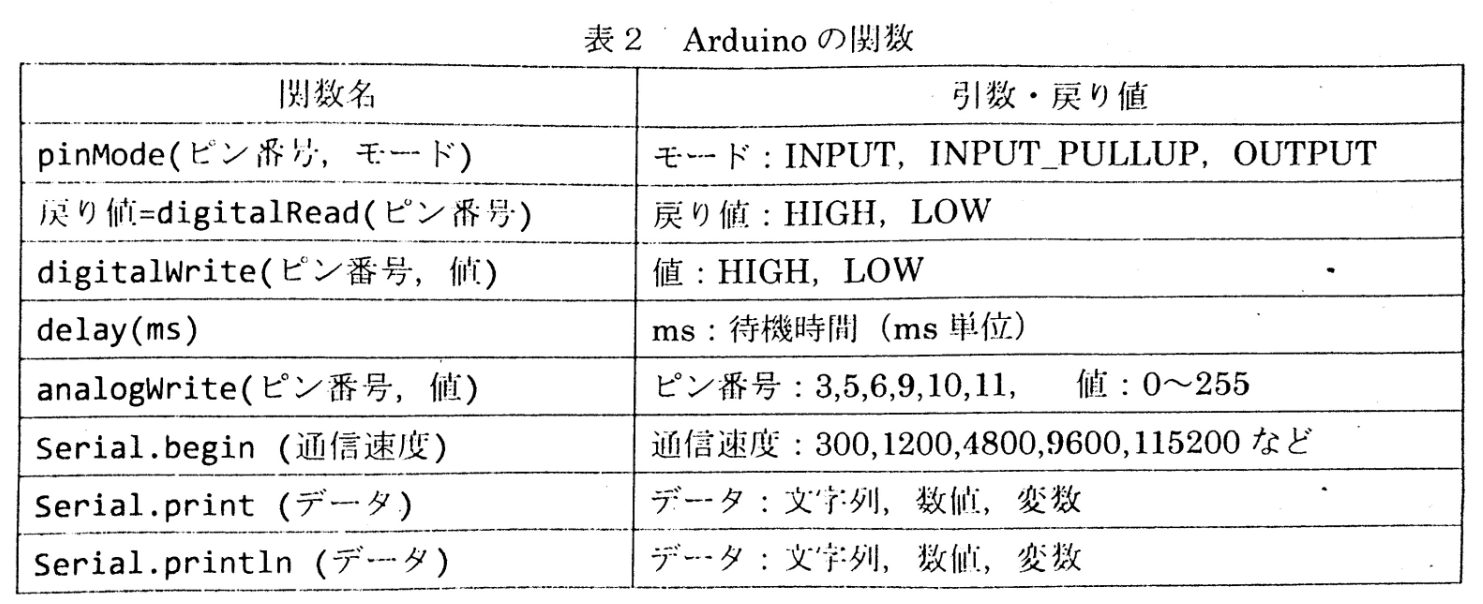
\includegraphics[width=0.88\linewidth]{image/MicroCon9.png}
\end{center}


\end{document}

